%!TEX root=../paper.tex

 % context-sensitive extension of PetitParser is used to define its grammar using parsing expressions

\section{Implementation}
Polite is implemented on top of Pharo Smalltalk. The language interpreter is built using a context-sensitive extension of PetitParser --- a parser combinator framework that uses the parsing expression grammar formalism \cite{Kurs14a-ParsingContext}. 

The current implementation of Polite can be found online and downloaded from  the Zenodo data repository \cite{kurs16-polite}. The repository contains an image which includes the code for the language implementation, a suite of more than 450 unit tests, and a sytax-highlighting code editor that is pictured in Figure 1. 

\begin{figure}[h]
	\centering
	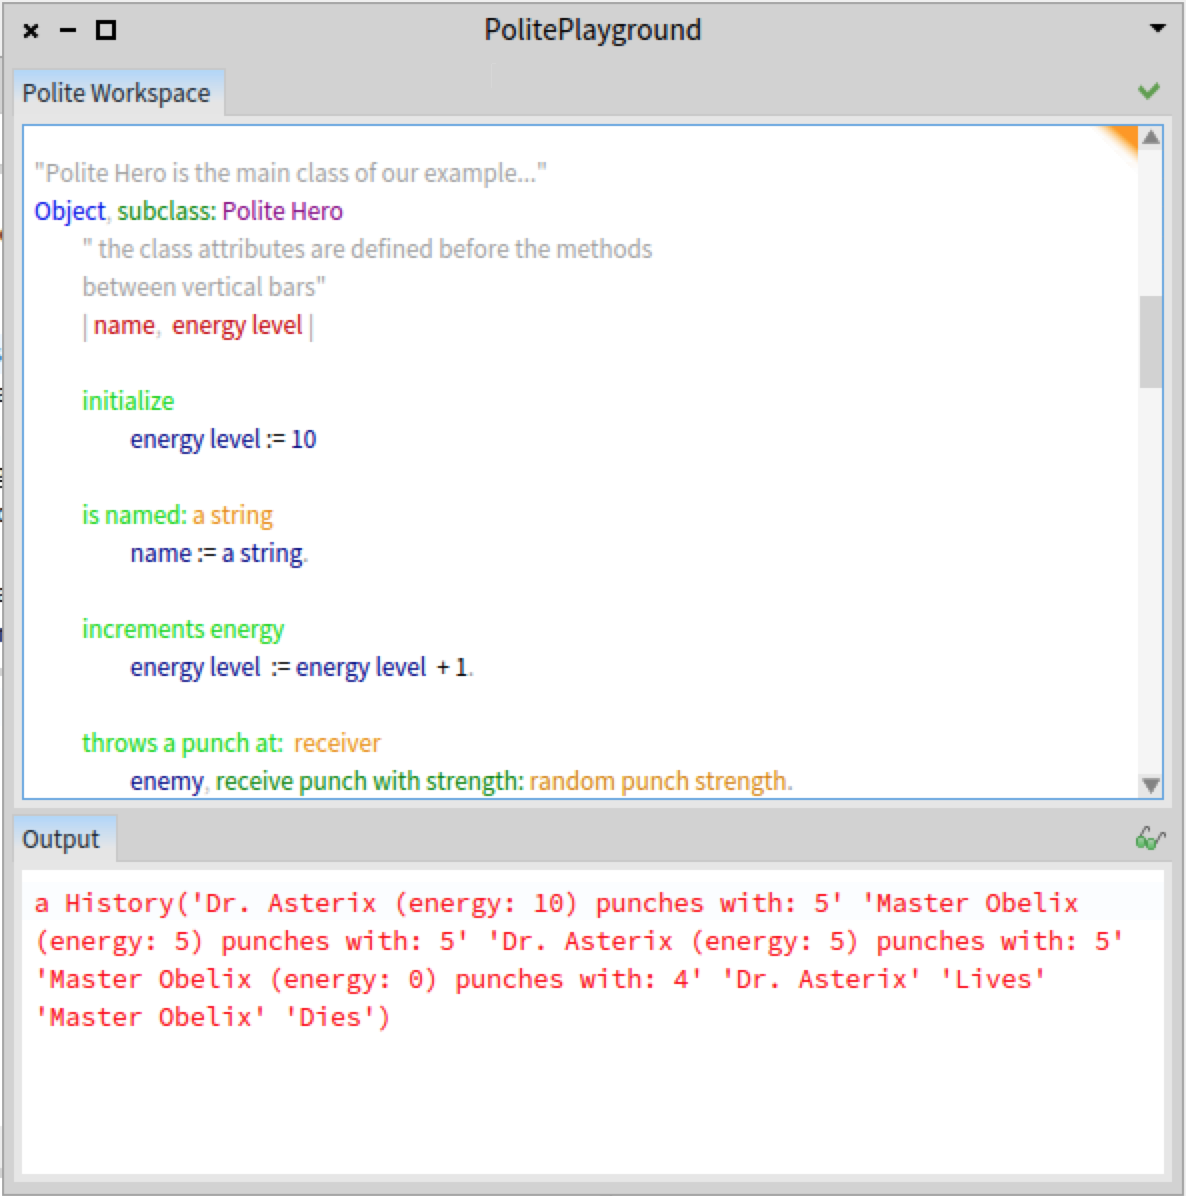
\includegraphics[width=0.45\textwidth]{images/playground.png}
	\caption{The Polite Playground provides a syntax highlighting code editor for Polite}
	\label{fig:figure1}
\end{figure}